\FloatBarrier
\section{Geometric preservation and functional consequences}\label{sec:mechanism}\label{sec:restoration}

We examine how PEFT methods change pretrained weight geometry and whether these changes are necessary for adaptation. We first explain singular-value and singular-basis changes theoretically, then measure spectral and hyperspherical energy preservation in checkpoints. Finally, we restore pretrained singular values to test whether adapted singular bases alone retain task gains.

\paragraph{Theoretical perspective.}
For $\bm W_0,\bm W_*\in\mathbb R^{m\times n}$, let $\bm W_j=\bm U_j\operatorname{diag}(\bm s_j)\bm V_j^{\!\top}$ denote thin SVDs with decreasing singular values, and let $O(k)$ denote the orthogonal group.
Relative weight and spectral displacement are defined by
$d_W={\|\bm W_*-\bm W_0\|_{\mathrm{F}}}/{\|\bm W_0\|_{\mathrm{F}}}$
and
$d_S={\|\bm s_*-\bm s_0\|_2}/{\|\bm s_0\|_2}$.

\begin{proposition}[Distance to the orthogonal orbit]\label{prop:orthogonal-distance}
The restored matrix $\bm W_R=\bm U_*\operatorname{diag}(\bm s_0)\bm V_*^{\!\top}$ satisfies
\begin{equation}\label{eq:orthogonal-distance}
\min_{\bm Q_L\in O(m),\,\bm Q_R\in O(n)}
\|\bm W_*-\bm Q_L\bm W_0\bm Q_R^{\!\top}\|_{\mathrm F}
=\|\bm W_*-\bm W_R\|_{\mathrm F}=\|\bm s_*-\bm s_0\|_2,
\end{equation}
and attains this minimum \citep{mirsky1975trace}. For nonzero base and update norms, $d_S/d_W$ is the distance to this orbit relative to the update norm.
\end{proposition}
We emphasize that the two-sided orbit in Proposition~\ref{prop:orthogonal-distance} is larger than OFT's one-sided right-orthogonal family. The proposition characterizes spectral preservation, not representability by OFT.

A small ratio means that changing the singular bases while keeping pretrained singular values closely approximates the adapted weights, with error measured relative to the update norm.

\begin{proposition}[First-order spectral and basis motion]\label{prop:first-order-motion}
Let $q=\min(m,n)$ and suppose $\bm W_0$ has $q$ distinct positive singular values. For $\bm W_*(\epsilon)=\bm W_0+\epsilon\bm E$, set $\dot{\bm s}=\left.\mathrm d\bm s(\epsilon)/\mathrm d\epsilon\right|_{\epsilon=0}$. Then
\begin{equation}\label{eq:tangent-normal}
\dot s_i=\bm u_{0,i}^{\!\top}\bm E\bm v_{0,i},\qquad
\bm E_N=\bm U_0\operatorname{diag}(\dot{\bm s})\bm V_0^{\!\top},\qquad
\bm E_T=\bm E-\bm E_N
\end{equation}
are the spectral derivative \citep{stewart1990}, the normal component and the tangent component to the two-sided orthogonal orbit, respectively. In particular, $\bm E_T$ changes only singular bases to first order, and $\|\bm E\|_{\mathrm F}^2=\|\dot{\bm s}\|_2^2+\|\bm E_T\|_{\mathrm F}^2$. If $\|\bm E\|_{\mathrm F}=1$ and $\mathbb E[\operatorname{vec}(\bm E)\operatorname{vec}(\bm E)^{\!\top}]=\bm I_{mn}/(mn)$, then
\begin{equation}\label{eq:relative-spectral-scale}
\mathbb E\|\dot{\bm s}\|_2^2=\frac{1}{\max(m,n)},\qquad
\lim_{\epsilon\to0}\sqrt{\mathbb E\left[\left(\frac{d_S}{d_W}\right)^2\right]}=\frac{1}{\sqrt{\max(m,n)}}.
\end{equation}
\end{proposition}
Small isotropic updates therefore have RMS $d_S/d_W\approx1/\sqrt{\max(m,n)}$: spectral displacement can be a small share of weight displacement without an orthogonality constraint. This conditional prediction also holds for uniformly oriented low-rank updates (proofs and pooling in Appendix~\ref{app:geometry}).

\paragraph{Empirical evaluation.}
At the largest capacities, spectral displacement is a modest fraction of weight displacement even for unconstrained methods (\Cref{fig:overview}b): about 11\% for Llama MiLoRA versus 3--4\% for LoRA, DoRA, and PiSSA, and 5.8\% and 8.7\% for FLUX PiSSA and MiLoRA, respectively.
We also measure hyperspherical energy (HE), whose preservation motivates OFT's approach to adaptation \citep{qiu2023oft}. For nonzero rows with distinct normalized directions, $H(\bm W)=\sum_{i\ne j}\|\widehat{\bm w}_i-\widehat{\bm w}_j\|_2^{-1}$, where $\widehat{\bm w}_i=\bm w_i/\|\bm w_i\|_2$. Right-orthogonal transformations preserve hyperspherical energy exactly, whereas preserving singular values alone does not. Nevertheless, all six methods approximately preserve HE: every checkpoint's mean absolute relative change across adapted matrices is below $0.01\%$ at the largest capacities (Appendix~\ref{app:hyperspherical}).
LoRA-family methods therefore approximately preserve both quantities without enforcing orthogonality. Their small spectral displacement further supports a two-sided orthogonal approximation of adapted weights (Proposition~\ref{prop:orthogonal-distance}). To assess the functional importance of singular-basis changes relative to singular-value scaling, we restore pretrained singular values while retaining adapted bases \citep{he2025posttrainingstructure,jin2026rlheals}.
Across LLM and FLUX checkpoints, all points at the largest capacities remain within one percentage point of reconstruction (\Cref{fig:overview}b). See Appendix~\ref{app:complete-interventions} for additional results at other capacities.
\begin{figure}[t]\centering
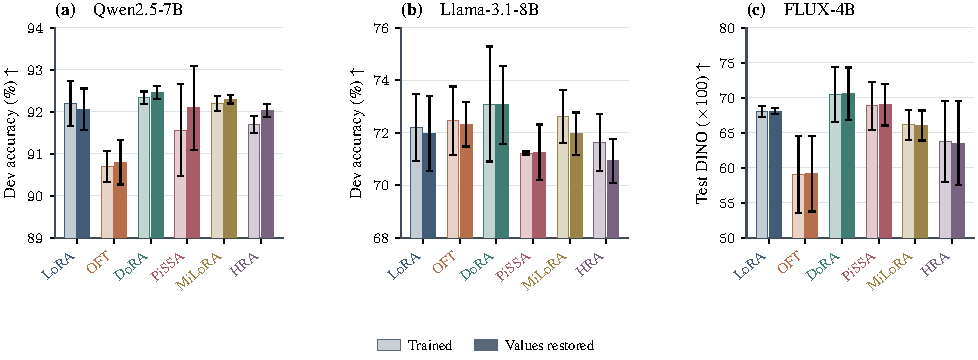
\includegraphics[width=\linewidth]{figures/peft_restoration.pdf}
\caption{Task performance largely survives singular-value restoration. At the largest capacities and development/validation-selected LRs, pale and saturated bars show trained and restored scores with sample SD error bars. LLM panels report development accuracy, and FLUX reports same-run test DINO for all six methods.}
\label{fig:restoration}
\end{figure}

\paragraph{Summary.}
In our settings, LoRA-family methods approximately preserve the spectra and hyperspherical energy that OFT is designed to preserve exactly. Singular-value restoration largely retains task performance. Tighter preservation must be judged by its task and retention outcomes.
